\vspace{-1em}
\subsection{Trust Nodes and Trust Functions}

\begin{figure}[htbp]
\centering
\begin{subfigure}{0.16\textwidth}
  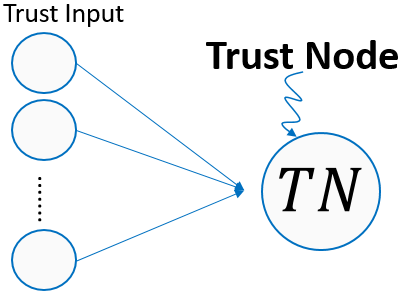
\includegraphics[width=\textwidth]{good_figs/trust_node/trustnode.png}
  \caption{Trust Node}
  \label{fig:tns}
\end{subfigure}
\hfill
\begin{subfigure}{0.27\textwidth}
  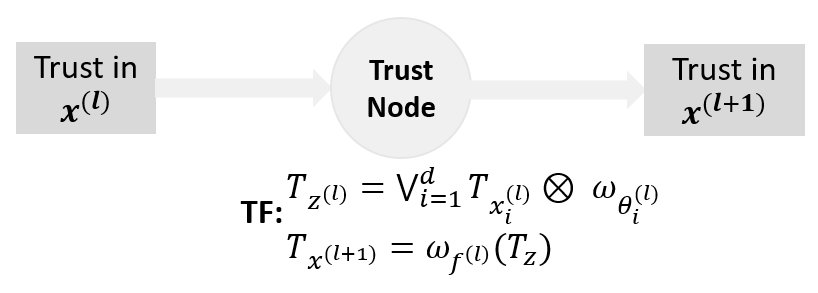
\includegraphics[width=\textwidth]{good_figs/trust_node/tnop.png}
  \caption{Trust Function operation}
  \label{fig:tnf}
\end{subfigure}
\caption{Trust Node structure and computation, mirroring the corresponding neuron (Appendix~\ref{app:trustnode}).}
\label{fig:trustnode}
\end{figure}

To extend \(\pf_\Theta\) from a single perceptron to larger networks, we introduce two fundamental concepts, the \emph{Trust Node} (\cref{fig:tns}) and the \emph{Trust Function} (\cref{fig:tnf}), which provide the basic mechanisms for propagating trust through the network structure. 

\begin{definition}[Trust Node]
A \emph{Trust Node} is an abstract computational unit associated with a neuron in a neural network. It receives trust opinions on the neuron’s inputs and produces a trust opinion on the neuron’s output. The structure of a Trust Node mirrors that of its corresponding neuron, but its computation is defined over trust opinions using operators such as discounting and fusion.
\end{definition}

\begin{definition}[Trust Function]\label{def:trustfunc}
A \emph{Trust Function} models the transformation of trust through a Trust Node. It defines how trust opinions on the inputs of a neuron are combined to produce a trust opinion on the output. 
For a neuron that computes
\(
z^{(l)} = \sum \theta^{(l)}_i \cdot x^{(l)}_i, \quad x^{(l+1)} = \phi^{(l)}(z^{(l)}),
\)
the corresponding trust computation is given by:
\begin{equation}
T_{z^{(l)}} = \bigoplus_{i=1}^{d} T_{x_{i}^{(l)}} \otimes T_{\theta_{i}^{(l)}}, \quad
T_{x^{(l+1)}} = T_{\phi^{(l)}}(T_{z^{(l)}}),
\label{eq:layerprop}
\end{equation}
where \( \otimes \) is a trust discounting operator, \(\bigoplus\) a trust fusion operator, and \( T_{\phi}^{(l)} \) the trust-equivalent of the activation function, set to the identity in this work since we use ReLU activations.
\end{definition}

As in \cref{eq:sol}, the discount operator \( \otimes \) models how trust in an input is modulated by trust in the associated parameter, while \( \bigoplus \) combines these contributions across inputs; fusion operators should be associative or generalizable~\cite{vanderheijden2018multisourcefusionoperationssubjective} to support multiple inputs. Reading the fused terms as opinions of distinct virtual sources about the same node output keeps this mapping algebraically consistent (Appendix~\ref{app:operators} gives the construction); this is precisely the consistency that variable-level fusion, as used in DeepTrust, lacks.

With these definitions in place, two challenges remain: quantifying the trustworthiness of parameters learned from datasets of variable quality, and generalizing trust propagation to deeper architectures. They motivate the Parallel Trust Assessment System (PaTAS), whose design, components, and theoretical foundations the next section presents.